\scanpage{82}
% archive foliation: 81
\[
\begin{array}{c|l}
\mathrm I&3\\
&7\ \unsure{\leftarrow}\ 9\\
&11\\
&12
\end{array}
\]
\margin{\unsure{total to} \unsure{all the} \unsure{implications}}
\margin{\fbox{\parbox{5cm}{ambiguity on points of formal schemes
quite general ---}}}

\deleted{\unsure{18|13} --- Most examples come from usual
\unsure{proper} schemes over $\mathbf Z$!}
\[
\begin{array}{l}
20\\27
\end{array}
\]

whole chapter looks plethoric

\[
\begin{array}{ll}
\mathrm{II}&2\\
&12\quad\text{unreasonable!}\\
&16\\&20\\&22
\end{array}
\]

\diagram{
\begin{tikzcd}[column sep=small,row sep=large]
& \boxed{\parbox{9cm}{explicit interpretation of $\pi_1^D$ in terms of
$\unsure{\mathfrak S}-\unsure{\operatorname{Supp}|\operatorname{Spec}}\,D$}}
\arrow[dl,leftrightarrow]\\
\boxed{\parbox{4cm}{whole chapter III seems to be used only to get
$\boxed{3.5.8}$}} &
\end{tikzcd}
}
\fbox{\parbox{10cm}{Copy of previous note on tame ramification?}}

\fbox{\parbox{10cm}{Include variant of Lefschetz's Theorem for $\pi_1^t$}}

\fbox{\parbox{10cm}{Include, after Mumford's theorem,
application to question of finite generation of local
\deleted{tame}\inserted{prime to $p$ ---} fund. group.}}

\[
\begin{array}{ll}
\underline{\mathrm{III}}&\underline{1}\\&2\\&6\quad\text{2 fois}\\&8\\&11\\&12^b
\end{array}
\]

16\quad add section on case when D.'s have equations!
This should make the situation much clearer!
For instance 3.4.1, 3.4.2

22

25\quad fppf descent for tamely ramified coverings?
At least one would like to have a ``champ'' on $\mathrm{Et}/S$!

26\quad \unsure{a)}\\
\hspace*{2em}\unsure{b)} Normality assumption more natural
(formal normality, \unsure{in loc.} formal schemes---)

28\quad\unsure{15}

\margin{cf 3.6.4}

Proof of $3.6.\unsure{5|8}$ is unbelievably long!

\figure{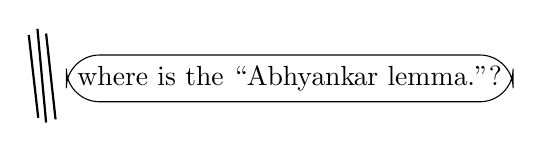
\begin{tikzpicture}[x=1cm,y=1cm]
\draw[line width=.8pt] (0,0)--(-.12,1.05) (.10,-.06)--(-.01,1.13) (.22,-.02)--(.10,1.07);
\node[draw,rounded corners=12pt,anchor=west,inner sep=4pt] at (.35,.5) {where is the ``Abhyankar lemma.''?};
\end{tikzpicture}}
